\documentclass[10pt]{beamer}

\usepackage[T2A]{fontenc}
\usepackage[utf8]{inputenc}
\usepackage[russian,english]{babel}

\usefonttheme[onlymath]{serif}

\usetheme[progressbar=frametitle]{metropolis}
\usepackage{appendixnumberbeamer}

\usepackage{booktabs}
\usepackage[scale=2]{ccicons}

\usepackage{pgfplots}
\usepgfplotslibrary{dateplot}

\usepackage{xspace}
\newcommand{\themename}{\textbf{\textsc{metropolis}}\xspace}
\newcommand{\TODO}[1]{\textbf{\textcolor{red}{TODO: #1}}}

\date{}
\author{Екатерина Тузова}

\usepackage{tikz}
\usetikzlibrary{arrows,positioning} 
\tikzset{
    mynode/.style={rectangle,rounded corners,draw=black, top color=white,very thick, inner sep=1em, text centered},
    mycircle/.style={circle,draw=black, top color=white,very thick, text centered},
    pil/.style={ ->, thick, shorten <=2pt, shorten >=2pt,}
}  

\title{Лекция 7}
\subtitle{Функционалы качества}

\begin{document}

\maketitle

\section{Разбор летучки}

\begin{frame}{Задача классификации}
  $X$ - множество объектов \\
	$Y$ - множество классов \\
	Обучающая выборка: ${X^l = (x_i, y_i)_{i=1}^l}$ \\ 
	Целевая функция: $f: X \rightarrow Y$\\
	\bigbreak
	Набор гипотез $h: X \rightarrow Y$, $h \in \mathcal{H}$ \\
	Алгоритм -- лучшая из гипотез $a: g \approx f$
\end{frame}

\begin{frame}{Модель}
  \begin{tikzpicture}[node distance=1cm, scale=0.8, transform shape]
    \node[mynode, text width=5cm] (target) 
      {Неизвестная целевая функция\\
      \textcolor{blue}{$f: X \rightarrow Y$}};
    \node[mynode, text width=3.5cm, below=1cm of target] (training) 
      {Обучающая выборка\\
      \textcolor{blue}{${X^l = (x_i, y_i)_{i=1}^l}$}}
          edge[pil, <-] (target.south);
    \node[below=1cm of training] (dummy) {}; 
    \onslide<2, 3>{    
      \node[mycircle,text width=1.5cm, below=1cm, right=2cm of dummy] (learning) 
        {Метод обучения\\
        \textcolor{blue}{$A$}}
        edge[pil, <-, bend left=15] (training.south);  
      }
    \onslide<3>{   
      \node[mynode, text width=3cm, below=1cm of dummy] (hypothesis) 
        {Набор гипотез\\
        \textcolor{blue}{$\mathcal{H}$}}
        edge[pil, bend left=15] (learning.west);  
        }
    \node[mynode, text width=3.5cm, right=1cm of learning] (final) 
      {Финальная гипотеза\\
      \textcolor{blue}{$a: g \approx f$}}
      edge[pil, <-] (learning.east);    
  \end{tikzpicture}
\end{frame}

\begin{frame}{Модель}
  \begin{tikzpicture}[node distance=1cm, scale=0.8, transform shape]
    \node[mynode, text width=5cm] (target) 
      {Неизвестная целевая функция\\
      \textcolor{blue}{$f: X \rightarrow Y$}};
    \node[mynode, text width=3.5cm, below=1cm of target] (training) 
      {Обучающая выборка\\
      \textcolor{blue}{${X^l = (x_i, y_i)_{i=1}^l}$}}
          edge[pil, <-] (target.south);
    \node[below=1cm of training] (dummy) {}; 
    \node[mycircle, orange, text width=1.5cm, below=1cm, right=2cm of dummy] (learning) 
      {Метод обучения\\
      \textcolor{blue}{$A$}}
      edge[pil, <-, bend left=15] (training.south);  
    \node[mynode, orange, text width=3cm, below=1cm of dummy] (hypothesis) 
      {Набор гипотез\\
      \textcolor{blue}{$\mathcal{H}$}}
      edge[pil, bend left=15] (learning.west);  
    \node[mynode, text width=3.5cm, right=1cm of learning] (final) 
      {Финальная гипотеза\\
      \textcolor{blue}{$a: g \approx f$}}
      edge[pil, <-] (learning.east);    
  \end{tikzpicture}
\end{frame}

\section{Пример}

\begin{frame}{Перцептрон}
  Набор гипотез:\\
  $h(\mathbf{x}) = \sign(\sum\limits_{j=1}^n {\only<2,3>{\color{orange}}w_j} x^j - {\only<2,3>{\color{orange}}w_0})$\\
  \bigbreak
  \pause
  \pause
  Метод обучения:\\
  \begin{algorithmic}[1]
        \Function{perceptron}{$X$}
            \State Инициализировать ${w_0, \dots, w_n}$
            \MRepeat [пока $w$ изменяются] 
               \For {$i = 1, \dots, l$}
                 \If {$a(x_i) \neq y_i$}
                   \State $w = w + y_i x_i$
                 \EndIf  
               \EndFor
           	\EndRepeat
        \EndFunction
    \end{algorithmic}
\end{frame}

\begin{frame}{Неравенство Бернштейна-Хёфдинга}
  \begin{minipage}[t]{0.5\linewidth}
    $$P[\vert \nu - \mu \vert < \varepsilon ] \leq 2 e^{-2 \varepsilon^2 l} $$\\
  \end{minipage}%
  \begin{minipage}{0.45\textwidth}
    \begin{center}
      \begin{figure}
        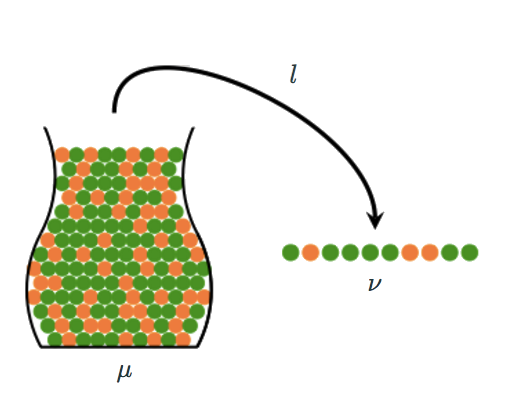
\includegraphics[width=\textwidth, keepaspectratio]{images/bin}    
      \end{figure}
    \end{center}

  \end{minipage}%
    \bigbreak
    $\nu$ -- доля оранжевых шаров в выборке размера $l$\\
    $\mu$ -- истинная доля оранжевых шаров в данных 
  
\end{frame}

\section{Какое отношение это имеет к нашим гипотезам?}

\begin{frame}
  Каждый шар это объект $x$ из пространства $X$.\\
  Неизвестная целевая функция $f$.\\
  \bigbreak
  Оранжевый шар -- гипотеза $h$ верна ($h(x) == f(x)$)\\
  Зелёный шар -- гипотеза $h$ не верна ($h(x) \neq f(x)$)\\
  \bigbreak
  По выборке $X^l$ можем оценить $\nu$ -- долю объектов, на которых верна гипотеза.
\end{frame}

\begin{frame}{Модель}
  \begin{tikzpicture}[node distance=1cm, scale=0.8, transform shape]
    \node[mynode, text width=5cm] (target) 
      {Неизвестная целевая функция\\
      \textcolor{blue}{$f: X \rightarrow Y$}};
    \node[mynode, text width=3.5cm, below=1cm of target] (training) 
      {Обучающая выборка\\
      \textcolor{blue}{${X^l = (}\textcolor{orange}{x_i}\textcolor{blue}{, y_i)_{i=1}^l}$}}
          edge[pil, <-] (target.south);
    \node[below=1cm of training] (dummy) {}; 
    \node[mycircle,text width=1.5cm, below=1cm, right=2cm of dummy] (learning) 
      {Метод обучения\\
      \textcolor{blue}{$A$}}
      edge[pil, <-, bend left=15] (training.south);  
    \node[mynode, text width=3cm, below=1cm of dummy] (hypothesis) 
      {Набор гипотез\\
      \textcolor{blue}{$\mathcal{H}$}}
      edge[pil, bend left=15] (learning.west);  
    \node[mynode, text width=3.5cm, right=1cm of learning] (final) 
      {Финальная гипотеза\\
      \textcolor{blue}{$a: g \approx f$}}
      edge[pil, <-] (learning.east);    
      
    \node[mynode, orange, right=1cm of target, text width=5cm] (probability) 
      {Вероятностное распределение\\
      \textcolor{blue}{$P$ на $X$}}
      edge[pil, bend left=35] (training.east);  
  \end{tikzpicture}
\end{frame}

\begin{frame}{$E_{in}$ и $E_{out}$}
  $E_{in}(h) = \nu$ - доля объектов в выборке $X^l$, на которых $h$ верна\\
  $E_{out}(h) = \mu$ - доля объектов во всём множестве $X$, на которых $h$ верна\\
  \bigbreak
  $$P[\vert E_{in}(h) - E_{out}(h) \vert < \varepsilon ] \leq 2 e^{-2 \varepsilon^2 l} $$\\
  \bigbreak
  Неравенство выполняется для каждой гипотезы.
\end{frame}

\begin{frame}{Важная деталь}
  \centering
  Какова вероятность, что гипотеза $a \in \mathcal{H}$, наилучшим образом приближающая $f$ по выборке, наилучшим образом приближает $f$ на всём множестве?
\end{frame}

\begin{frame}{Простая аналогия}
  \centering
  С какой вероятностью монета, подброшенная 10 раз, выпадет одной и той же стороной все 10 раз?
  \pause
  \bigbreak
  \textcolor{blue}{$0.001$}
\end{frame}

\begin{frame}{Простая аналогия}
  \centering
  С какой вероятностью одна из 1000 монет, каждая из которых подброшена 10 раз, выпадет одной и той же стороной все 10 раз?
  \pause
  \bigbreak
  \textcolor{blue}{$0.63$}
\end{frame}

\begin{frame} {К нашей задаче}
  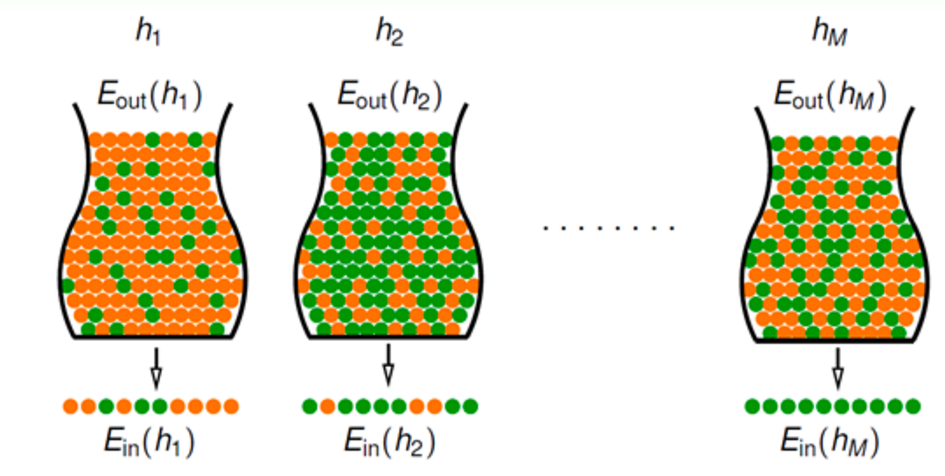
\includegraphics[width=\textwidth, keepaspectratio]{images/bins}
\end{frame}

\begin{frame} {Решение}
  \begin{align*}
    P[\vert E_{in}(a) - E_{out}(a) \vert < \varepsilon ] &\leq \sum\limits_{m=1}^M P[\vert E_{in}(h) - E_{out}(h) \vert < \varepsilon ] \\
    & \leq 2\textcolor{orange}{M} e^{-2 \varepsilon^2 l} 
  \end{align*}
\end{frame}

%{\foot{loss function}
%\begin{frame}{Функция потерь}
%  Функция потерь $\mathcal{L}(a, x_i) $ -- характеризует величину ошибки алгоритма $a$ на объекте $x_i$.\\
%  \bigbreak
%  Если $\mathcal{L} (a, x_i) = 0$, то ответ $a(x_i)$ называется корректным.
%\end{frame}
%}

{\foot{loss function}
\begin{frame}{Функция потерь}
  Задача классификации:\\
  $\mathcal{L}(h, x_i) = [h(x_i) \neq y_i]$ -- индикатор ошибки\\
  \bigbreak
  Задача регрессии:\\
  $\mathcal{L}(h, x_i) = \vert h(x_i) - y_i \vert$ -- абсолютное значение ошибки\\
  $\mathcal{L}(h, x_i) = (h(x_i) - y_i)^2$ -- квадратичная ошибка\\
\end{frame}
}

{\foot{функционал средних потерь, Empirical Risk}
\begin{frame}{Функционал качества}
  Функционал качества гипотезы $h$ на выборке $X^l$:\\
  $$E_{in}(h, X^l) = \frac{1}{l} \sum\limits_{i=1}^l \mathcal{L}(h, x_i)$$\\
  Минимизация эмпирического риска:\\
  $$\arg\min\limits_{h} E_{in}(h, X^l)$$
\end{frame}
}

\begin{frame}{Полная и поточечная ошибка}  
  $$E_{in}(h, X^l) = \frac{1}{l} \sum\limits_{i=1}^l \mathcal{L}(h, x_i)$$\\
  \bigbreak
  $$E_{out} = \mathbb{E}_x \mathcal{L}(h, x_i) $$
\end{frame}

\begin{frame}{Шум в наблюдениях}  

\end{frame}

\begin{frame}[standout]
  Вопросы?
\end{frame}

\appendix

\begin{frame}\frametitle{На следующей лекции}
	\begin{itemize}
    	\item[--] Функционалы качества
    	\item[--] Неравенство Хефдинга
    	\item[--] Близость гипотез
    	\item[--] Неравенство Вапника-Червоненкиса
    	\item[--] Генерация модельных данных    	    	
	\end{itemize}
\end{frame}
\end{document}

\end{document}